\documentclass[border=10pt]{standalone}
\usepackage{tikz}
\usetikzlibrary{arrows.meta, positioning, shapes.geometric, calc}

\begin{document}
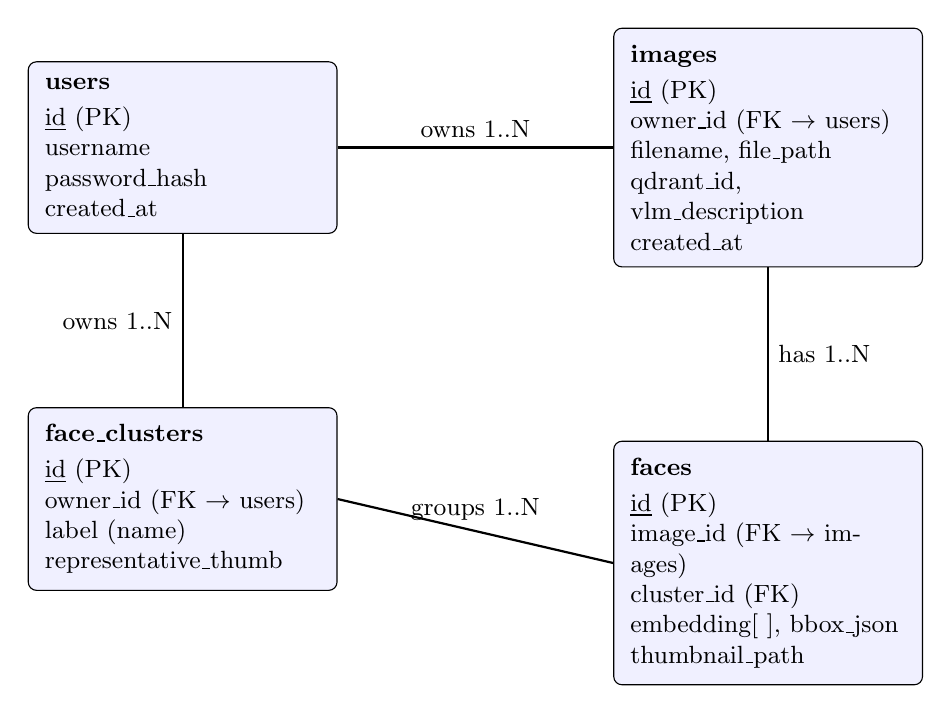
\begin{tikzpicture}[
  node distance=1.0cm and 3.5cm,
  ent/.style={draw, rectangle, rounded corners=3pt, fill=blue!6,
              text width=3.5cm, align=left, font=\small,
              inner sep=6pt},
  arr/.style={-, thick},
]
\node[ent] (u) {
  \textbf{users}\\[2pt]
  \underline{id} (PK)\\username\\password\_hash\\created\_at
};
\node[ent, right=3.5cm of u] (img) {
  \textbf{images}\\[2pt]
  \underline{id} (PK)\\owner\_id (FK $\to$ users)\\filename, file\_path\\qdrant\_id, vlm\_description\\created\_at
};
\node[ent, below=2.2cm of img] (f) {
  \textbf{faces}\\[2pt]
  \underline{id} (PK)\\image\_id (FK $\to$ images)\\cluster\_id (FK)\\embedding[ ], bbox\_json\\thumbnail\_path
};
\node[ent, below=2.2cm of u] (fc) {
  \textbf{face\_clusters}\\[2pt]
  \underline{id} (PK)\\owner\_id (FK $\to$ users)\\label (name)\\representative\_thumb
};
%% Relationships
\draw[arr] (u.east)    -- node[above, font=\small]{owns 1..N}   (img.west);
\draw[arr] (img.south) -- node[right, font=\small]{has 1..N}    (f.north);
\draw[arr] (fc.east)   -- node[above, font=\small]{groups 1..N} (f.west);
\draw[arr] (u.south)   -- node[left,  font=\small]{owns 1..N}   (fc.north);
\end{tikzpicture}
\end{document}
